\chapter{Variational Autoencoders}

\textbf{Prerequisites} : \href{./13.md}{Ch A. Appendix - Basics of Monte Carlo}

\begin{concept}[11.1][Math Review]
    Let $A$ and $B$ be probabilistic events. Assume $A$ has nonzero probability.

    \textbf{Conditional probability} satisfies

    $$
    \mathbb{P}(B \mid A) \mathbb{P}(A)=\mathbb{P}(A \cap B)
    $$

    \textbf{Bayes' theorem} is an application of conditional probability:

    $$
    \mathbb{P}(B \mid A)=\frac{\mathbb{P}(A \mid B) \mathbb{P}(B)}{\mathbb{P}(A)}
    $$
\end{concept}

\begin{concept}[11.2][Math Review]
    Let $X \in \mathbb{R}^{m}$ and $Z \in \mathbb{R}^{n}$ be continuous random variables with joint density $p(x, z)$.

    The marginal densities are defined by

    $$
    p_{X}(x)=\int_{\mathbb{R}^{n}} p(x, z) d z, \quad p_{Z}(z)=\int_{\mathbb{R}^{m}} p(x, z) d x
    $$

    The conditional density function $p(z \mid x)$ has the following properties

    $$
    \begin{gathered}
    \mathbb{P}(Z \in S \mid X=x)=\int_{S} p(z \mid x) d z \\
    p(z \mid x) p_{X}(x)=p(x, z), \quad p(z \mid x)=\frac{p(x \mid z) p_{Z}(z)}{p_{X}(x)}
    \end{gathered}
    $$
\end{concept}

\begin{concept}[11.3][Introduction for Variational Autoencoders (VAE)]
    Key idea of \textbf{VAE}:

    \begin{itemize}
        \item \textbf{Latent variable model} with conditional probability distribution represented by $p_{\theta}(x \mid z)$.
        \item Efficiently estimate $p_{\theta}(x)=\mathbb{E}_{Z \sim p_{Z}}\left[p_{\theta}(x \mid Z)\right]$ by \textbf{importance sampling} with $Z \sim q_{\phi}(z \mid x)$.
    \end{itemize}

    We can interpret $q_{\phi}(z \mid x)$ as an encoder and $p_{\theta}(x \mid z)$ as a decoder.

    VAEs differ from autoencoders as follows:

    \begin{itemize}
        \item Derivations (latent variable model vs. dimensionality reduction)
        \item VAE regularizes/controls latent distribution, while AE does not.
    \end{itemize}
\end{concept}

\begin{figure}[H]
    \centering
    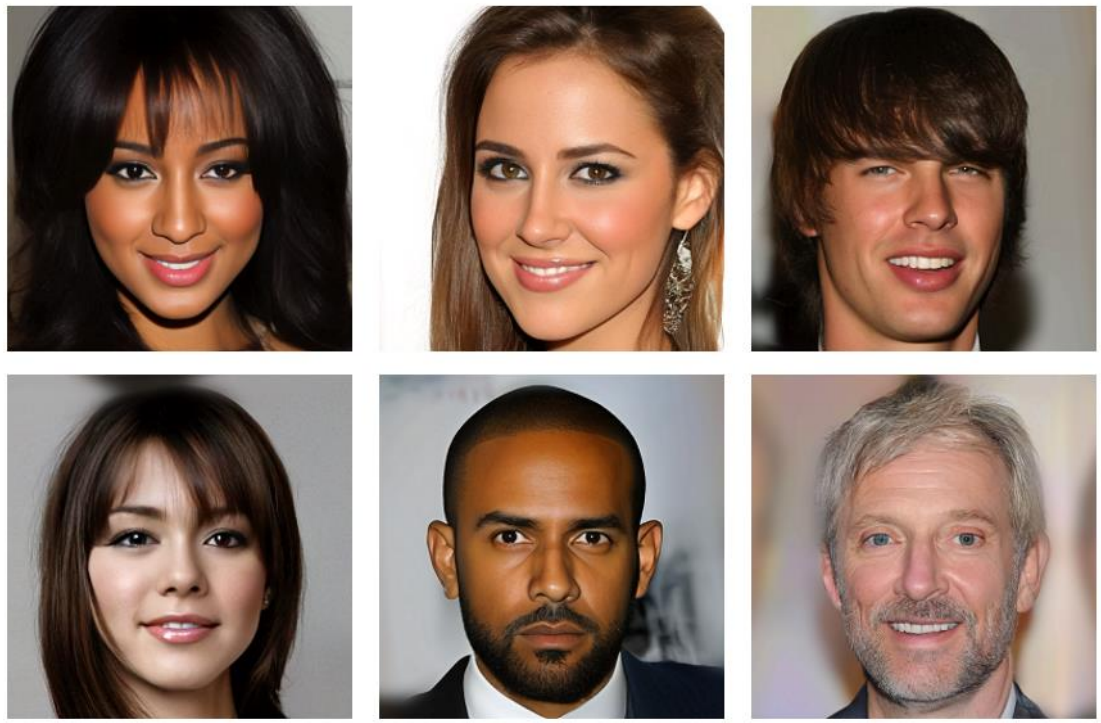
\includegraphics[width=0.8\textwidth]{.././assets/11.1.png}
\end{figure}

These are synthetic (fake) images made with VAE.

(A. Vahdat and J. Kautz, NVAE: A deep hierarchical variational autoencoder, NeurIPS, 2020.)

\section{Latent Variable Model}

\begin{itemize}
    \item
    Assumption on data $X_{1}, \ldots, X_{N}$

    Assumes there is an underlying latent variable $Z$ representing the "essential structure" of the data and an observable variable $X$ which generation is conditioned on $Z$. Implicitly assumes the conditional randomness of $X \sim p_{X \mid Z}$ is significantly smaller than the overall randomness $X \sim p_{X}$.
    \item
    Example

    $X$ is a cat picture. $Z$ encodes information about the body position, fur color, and facial expression of a cat. Latent variable $Z$ encodes the overall content of the image, but $X$ does contain details not specified in $Z$.
\end{itemize}

\begin{definition}[11.4][Latent Variable Model]
    VAEs implements a \textbf{latent variable model} with a NN that generates $X$ given $Z$. More precisely, NN is a deterministic function that outputs the conditional distribution $p_{\theta}(x \mid Z)$, and $X$ is randomly generated according to this distribution. This structure may effectively learn the latent structure from data if the assumption on data is accurate.

    \par\noindent\textcolor{gray}{\hdashrule{\textwidth}{0.4pt}{1pt 2pt}}

    \begin{figure}[H]
        \centering
        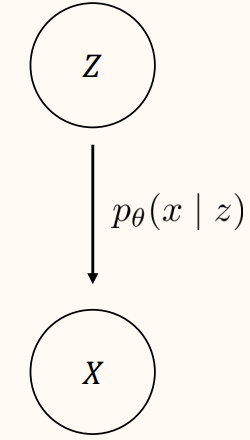
\includegraphics[width=0.2\textwidth]{.././assets/11.2.png}
    \end{figure}

    Sampling process:

    $$
    X \sim p_{\theta}(x \mid Z), \quad Z \sim p_{Z}(z)
    $$

    Usually $p_{Z}$ is a Gaussian (fixed) and $p_{\theta}(x \mid z)$ is a NN parameterized by $\theta$.

    Evaluating density (likelihood):

    $$
    p_{\theta}\left(X_{i}\right)=\int_{z} p_{Z}(z) p_{\theta}\left(X_{i} \mid z\right) d z=\mathbb{E}_{Z \sim p_{Z}}\left[p_{\theta}\left(X_{i} \mid Z\right)\right]
    $$

    Training via MLE:

    $$
    \underset{\theta \in \Theta}{\operatorname{maximize}} \sum_{i=1}^{N} \log p_{\theta}\left(X_{i}\right)=\underset{\theta \in \Theta}{\operatorname{maximize}} \sum_{i=1}^{N} \log \mathbb{E}_{Z \sim p_{Z}}\left[p_{\theta}\left(X_{i} \mid Z\right)\right]
    $$

    \par\noindent\textcolor{gray}{\hdashrule{\textwidth}{0.4pt}{1pt 2pt}}

    When $p_{Z}$ is a discrete:

    $$
    p_{\theta}(x)=\mathbb{E}_{Z \sim p_{Z}}\left[p_{\theta}(x \mid Z)\right]=\sum_{z} p_{Z}(z) p_{\theta}(x \mid Z)
    $$

    When $p_{Z}$ is a continuous:

    $$
    p_{\theta}(x)=\mathbb{E}_{Z \sim p_{Z}}\left[p_{\theta}(x \mid Z)\right]=\int_{z} p_{Z}(z) p_{\theta}(x \mid z) d z
    $$

    To clarify, specification of $p_{Z}(z)$ and $p_{\theta}(x \mid z)$ fully determines $p_{\theta}(x)$ (as above) and

    $$
    p_{\theta}(z \mid x)=\frac{p_{\theta}(x \mid z) p_{Z}(z)}{p_{\theta}(x)}
    $$

    \par\noindent\textcolor{gray}{\hdashrule{\textwidth}{0.4pt}{1pt 2pt}}

    Training

    $$
    \underset{\theta \in \Theta}{\operatorname{maximize}} \sum_{i=1}^{N} \log p_{\theta}\left(X_{i}\right)=\underset{\theta \in \Theta}{\operatorname{maximize}} \sum_{i=1}^{N} \log \mathbb{E}_{Z \sim p_{Z}}\left[p_{\theta}\left(X_{i} \mid Z\right)\right]
    $$

    requires evaluation $\mathbb{E}_{Z}$.

    \begin{itemize}
        \item Scenario 1: If $Z$ is discrete and takes a few of values, then compute $\sum_{z}$ exactly.
        \item Scenario 2: If $Z$ takes many values or if it is a continuous, then $\sum_{z}$ or $\mathbb{E}_{Z}$ is impractical to compute. In this case, approximate expectation with Monte Carlo and importance sampling.
    \end{itemize}
\end{definition}

\begin{example}[11.5][Example Latent Variable Model]
    Mixture of 3 Gaussians in $\mathbb{R}^{2}$, uniform prior over components. (We can make the mixture weights a trainable parameter.)

    $$
    \begin{gathered}
    p_{Z}(Z=A)=p_{Z}(Z=B)=p_{Z}(Z=C)=\frac{1}{3} \\
    p_{\theta}(x \mid Z=k)=\frac{1}{2 \pi\left|\Sigma_{k}\right|^{\frac{1}{2}}} \exp \left(-\frac{1}{2}\left(x-\mu_{k}\right)^{\top} \Sigma_{k}^{-1}\left(x-\mu_{k}\right)\right)
    \end{gathered}
    $$

    Training objective:

    $$
    \begin{aligned}
    \underset{\mu, \Sigma}{\operatorname{maximize}} \sum_{i=1}^{N} \log p_{\theta}\left(X_{i}\right)=\underset{\mu, \Sigma}{\operatorname{maximize}} \sum_{i=1}^{N} \log & \left[ \frac{1}{3} \frac{1}{2 \pi\left|\Sigma_{A}\right|^{\frac{1}{2}}} \exp \left(-\frac{1}{2}\left(X_{i}-\mu_{A}\right)^{\top} \Sigma_{A}^{-1}\left(X_{i}-\mu_{A}\right)\right) \right.\\
    & +\frac{1}{3} \frac{1}{2 \pi\left|\Sigma_{B}\right|^{\frac{1}{2}}} \exp \left(-\frac{1}{2}\left(X_{i}-\mu_{B}\right)^{\top} \Sigma_{B}^{-1}\left(X_{i}-\mu_{B}\right)\right) \\
    & \left.+\frac{1}{3} \frac{1}{2 \pi\left|\Sigma_{C}\right|^{\frac{1}{2}}} \exp \left(-\frac{1}{2}\left(X_{i}-\mu_{C}\right)^{\top} \Sigma_{C}^{-1}\left(X_{i}-\mu_{C}\right)\right)\right]
    \end{aligned}
    $$

    \begin{figure}[H]
        \centering
        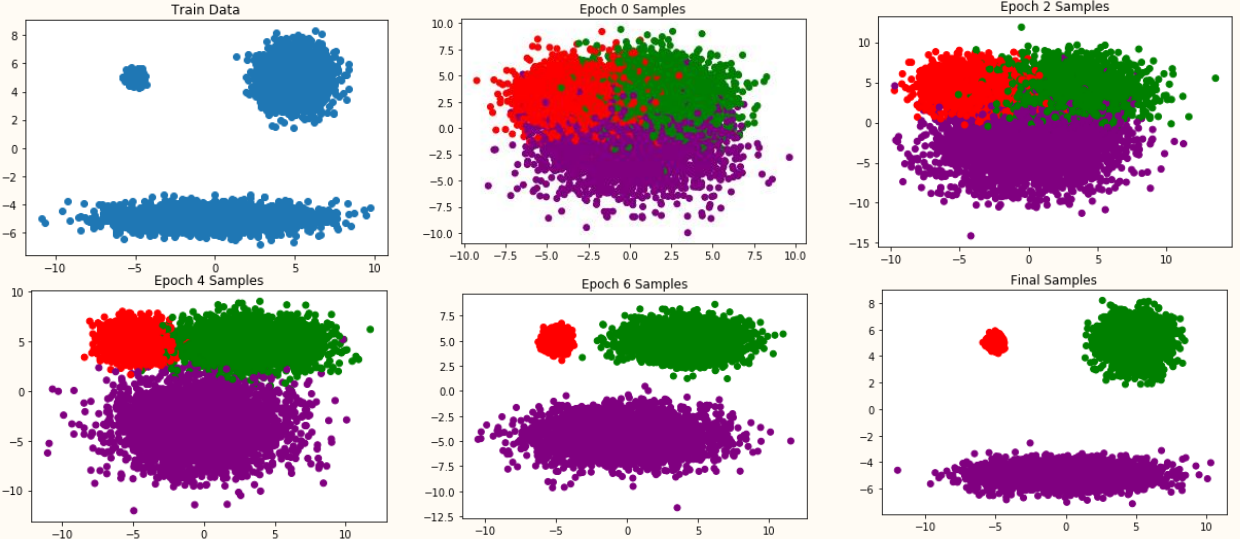
\includegraphics[width=1.0\textwidth]{.././assets/11.3.png}
    \end{figure}
\end{example}

\section{Training Latent Variable Model with Importance Sampling}

From now on, we will focus on \textbf{HOW} to train latent variable model with MLE,

$$
\underset{\theta \in \Theta}{\operatorname{maximize}} \sum_{i=1}^{N} \log p_{\theta}\left(X_{i}\right)=\underset{\theta \in \Theta}{\operatorname{maximize}} \sum_{i=1}^{N} \log \mathbb{E}_{Z \sim p_{Z}}\left[p_{\theta}\left(X_{i} \mid Z\right)\right]
$$

\begin{concept}[11.6][VAE Outline]
    Outline of variational autoencoder (VAE):

    \begin{enumerate}
        \item
        (Choice 1) Approximate intractable objective with a single $Z$ sample

        $$
        \sum_{i=1}^{N} \log \mathbb{E}_{Z \sim p_{Z}}\left[p_{\theta}\left(X_{i} \mid Z\right)\right] \approx \sum_{i=1}^{N} \log p_{\theta}\left(X_{i} \mid Z_{i}\right), \quad Z_{i} \sim p_{Z}
        $$
        \item
        (Choice 2) Improve accuracy of approximation by sampling $Z_{i}$ with importance sampling

        $$
        \sum_{i=1}^{N} \log \mathbb{E}_{Z \sim p_{Z}}\left[p_{\theta}\left(X_{i} \mid Z\right)\right] \approx \sum_{i=1}^{N} \log \frac{p_{\theta}\left(X_{i} \mid Z_{i}\right) p_{Z}\left(Z_{i}\right)}{q_{i}\left(Z_{i}\right)}, \quad Z_{i} \sim q_{i}
        $$
        \item Optimize approximate objective with SGD.
    \end{enumerate}

    (D. Kingma and M. Welling, VAE: Auto-encoding variational Bayes, ICLR, 2014.)
\end{concept}

\begin{concept}[11.7][IWAE Outline]
    Importance weighted autoencoders (IWAE) approximates intractable with $K$ samples of $Z$ :

    $$
    \sum_{i=1}^{N} \log \mathbb{E}_{Z \sim p_{Z}}\left[p_{\theta}\left(X_{i} \mid Z\right)\right] \approx \sum_{i=1}^{N} \log \frac{1}{K} \sum_{k=1}^{K} \frac{p_{\theta}\left(X_{i} \mid Z_{i, k}\right) p_{Z}\left(Z_{i, k}\right)}{q_{i}\left(Z_{i, k}\right)}, \quad Z_{i, 1}, \ldots, Z_{i, K} \sim q_{i}
    $$

    (Y. Burda, R. Grosse, and R. Salakhutdinov, Importance weighted autoencoders, ICLR, 2016.)
\end{concept}

\begin{concept}[11.8][Why does VAE need IS?]
    Among the two choices given in \hyperref[concept:11.6]{Concept 11.6}, VAEs improve the accuracy of latent variable model with IS (Choice 2).

    Sampling $Z_{i} \sim p_{Z}$ (Choice 1) results in a high-variance estimator:

    $$
    \mathbb{E}_{Z \sim p_{Z}}\left[p_{\theta}\left(X_{i} \mid Z\right)\right] \approx p_{\theta}\left(X_{i} \mid Z_{i}\right),
    $$

    In the Gaussian mixture example (\hyperref[example:11.5]{Example 11.5}), only $1 / 3$ of the $Z$ samples meaningfully contribute to the estimate. More specifically, if $X_{i}$ is near $\mu_{A}$ but is far from $\mu_{B}$ and $\mu_{C}$, then $p_{\theta}\left(X_{i} \mid Z=A\right) \gg 0$ but $p_{\theta}\left(X_{i} \mid Z=B\right) \approx 0$ and $p_{\theta}\left(X_{i} \mid Z=C\right) \approx 0$.

    The issue worsens as the observable and latent variable dimension increases.
\end{concept}

\par\noindent\textcolor{gray}{\hdashrule{\textwidth}{0.4pt}{1pt 2pt}}

\begin{concept}[11.9][Naïve Approach]
    To improve estimation of $\mathbb{E}_{Z \sim p_{Z}}\left[p_{\theta}\left(X_{i} \mid Z\right)\right]$, consider importance sampling (IS) with sampling distribution $Z_{i} \sim q_{i}(z)$ :

    $$
    \mathbb{E}_{Z \sim p_{Z}}\left[p_{\theta}\left(X_{i} \mid Z\right)\right] \approx p_{\theta}\left(X_{i} \mid Z_{i}\right) \frac{p_{Z}\left(Z_{i}\right)}{q_{i}\left(Z_{i}\right)}
    $$

    Optimal IS sampling distribution

    $$
    q_{i}^{\star}(z)=\frac{p_{\theta}\left(X_{i} \mid z\right) p_{Z}(z)}{\textcolor{red}{p_{\theta}\left(X_{i}\right)}}=\textcolor{red}{p_{\theta}\left(z \mid X_{i}\right)}
    $$

    To clarify, optimal sampling distribution depends on $X_{i}$.
    To clarify, $\textcolor{red}{p_{\theta}\left(X_{i}\right)}$ is the unkown normalizing factor so $\textcolor{red}{p_{\theta}\left(z \mid X_{i}\right)}$ is also unkown.
    We call $q_{i}^{\star}(z)=p_{\theta}\left(z \mid X_{i}\right)$ the true \textbf{posterior} distribution and we will soon consider the approximation $q_{\phi}(z \mid x) \approx p_{\theta}(z \mid x)$, which we call the \textbf{approximate posterior}.

    \par\noindent\textcolor{gray}{\hdashrule{\textwidth}{0.4pt}{1pt 2pt}}

    For each $X_{i}$, let $q_i(z)$ be the optimal approximate posterior dependent on $X_i$, and consider

    $$
    \begin{gathered}
    \underset{q_{i}}{\operatorname{minimize}} D_{\mathrm{KL}}\left(q_{i}(\cdot) \| \textcolor{red}{p_{\theta}\left(\cdot \mid X_{i}\right)} \right)\\
    =\underset{q_{i}}{\operatorname{minimize}} \mathbb{E}_{Z \sim q_{i}} \log \left(\frac{q_{i}(Z)}{\textcolor{red}{p_{\theta}\left(Z \mid X_{i}\right)}}\right) \\
    =\underset{q_{i}}{\operatorname{minimize}} \mathbb{E}_{Z \sim q_{i}} \log \left(\frac{q_{i}(Z)}{p_{\theta}\left(X_{i} \mid Z\right) p_{Z}(Z) / \textcolor{red}{p_{\theta}\left(X_{i}\right)}}\right) \\
    =\underset{Z \sim q_{i}}{\operatorname{minimize}}\left[\log q_{i}(Z)-\log p_{Z}(Z)-\log p_{\theta}\left(X_{i} \mid Z\right)\right]+\textcolor{red}{\log p_{\theta}\left(X_{i}\right)}
    \end{gathered}
    $$

    Note, $q_{i}(z), p_{Z}(z)$, and $p_{\theta}(x \mid z)$ are tractable/known while $\textcolor{red}{p_{\theta}\left(X_{i}\right)}$ and $\textcolor{red}{p_{\theta}\left(z \mid X_{i}\right)}$ are intractable/unknown. Since $\textcolor{red}{\log p_{\theta}\left(X_{i}\right)}$ does not depend on $q_{i}$, all quantities needed in the optimization problems are tractable. However, solving this minimization problem to obtain each $q_{i}$ for each data point $X_{i}$ is computationally too expensive.

    \par\noindent\textcolor{gray}{\hdashrule{\textwidth}{0.4pt}{1pt 2pt}}

    Individual inference (not amortized): For each $X_{1}, \ldots, X_{N}$, find corresponding optimal $q_{1}, \ldots, q_{N}$ by solving

    $$
    \underset{q_{i}}{\operatorname{minimize}} \quad D_{\mathrm{KL}}\left(q_{i}(\cdot) \| p_{\theta}\left(\cdot \mid X_{i}\right)\right)
    $$

    This is expensive as it requires solving $N$ separate optimization problems.

    We need variational approach and amortized inference.
\end{concept}

\begin{concept}[11.10][Variational Approach and Amortized Inference]
    General principle of variational approach: We can't directly use the $q$ we want. So, instead, we propose a parameterized distribution $q_{\phi}$ that we can work with easily (in this case, sample from easily), and find a parameter setting that makes it as good as possible.

    Parametrization of VAE:

    $$
    q_{\phi}\left(z \mid X_{i}\right) \approx q_{i}^{\star}(z)=p_{\theta}\left(z \mid X_{i}\right) \quad \text { for all } i=1, \ldots, N
    $$

    Amortized inference: Train a neural network $q_{\phi}(\cdot \mid x)$ such that $q_{\phi}\left(\cdot \mid X_{i}\right)$ approximates the optimal $q_{i}(\cdot)$.

    $$
    \underset{\phi \in \Phi}{\operatorname{minimize}} \sum_{i=1}^{N} D_{\mathrm{KL}}\left(q_{\phi}\left(\cdot \mid X_{i}\right) \| p_{\theta}\left(\cdot \mid X_{i}\right)\right)
    $$

    Approximation $q_{\phi}\left(z \mid X_{i}\right) \approx p_{\theta}\left(z \mid X_{i}\right)$ is often less precise than that of individual inference $q_{i}(z) \approx$ $p_{\theta}\left(z \mid X_{i}\right)$, but amortized inference is often significantly faster.
\end{concept}

\begin{concept}[11.11][Encoder $q_{\phi}$ Optimization]
    In analogy with autoencoders, we call $q_{\phi}$ the \textbf{encoder}.

    Optimization problem for encoder (derived from \hyperref[concept:11.9]{Concept 11.9}) :

    $$
    \begin{aligned}
    & \underset{\phi \in \Phi}{\operatorname{minimize}} \sum_{i=1}^{N} D_{\mathrm{KL}}\left(q_{\phi}\left(\cdot \mid X_{i}\right) \| p_{\theta}\left(\cdot \mid X_{i}\right)\right) \\
    = & \underset{\phi \in \Phi}{\operatorname{maximize}} \sum_{i=1}^{N} \mathbb{E}_{Z \sim q_{\phi}\left(z \mid X_{i}\right)}\left[\log \left(\frac{p_{\theta}\left(X_{i} \mid Z\right) p_{Z}(Z)}{q_{\phi}\left(Z \mid X_{i}\right)}\right)\right]+\text { constant independent of } \phi \\
    = & \underset{\phi \in \Phi}{\operatorname{maximize}} \sum_{i=1}^{N} \mathbb{E}_{Z \sim q_{\phi}\left(z \mid X_{i}\right)}\left[\log p_{\theta}\left(X_{i} \mid Z\right)\right]-D_{\mathrm{KL}}\left(q_{\phi}\left(\cdot \mid X_{i}\right) \| p_{Z}(\cdot)\right)
    \end{aligned}
    $$
\end{concept}

\begin{concept}[11.12][Decoder $p_{\theta}$ Optimization]
    In analogy with autoencoders, we call $p_{\theta}$ the \textbf{decoder}.
    Perform approximate MLE (derived from IS, Choice 2 of \hyperref[concept:11.6]{Concept 11.6}) :

    $$
    \begin{aligned}
    & \underset{\theta \in \Theta}{\operatorname{maximize}} \sum_{i=1}^{N} \log p_{\theta}\left(X_{i}\right)=\underset{\theta \in \Theta}{\operatorname{maximize}} \sum_{i=1}^{N} \log \mathbb{E}_{Z \sim p_{Z}}\left[p_{\theta}\left(X_{i} \mid Z\right)\right] \\
    \stackrel{(a)}{\approx} & \underset{\theta \in \Theta}{\operatorname{maximize}} \sum_{i=1}^{N} \log \left(\frac{p_{\theta}\left(X_{i} \mid Z_{i}\right) p_{Z}\left(Z_{i}\right)}{q_{\phi}\left(Z_{i} \mid X_{i}\right)}\right), \quad Z_{i} \sim q_{\phi}\left(z \mid X_{i}\right) \\
    \stackrel{(b)}{\approx} & \underset{\theta \in \Theta}{\operatorname{maximize}} \sum_{i=1}^{N} \mathbb{E}_{Z \sim q_{\phi}\left(z \mid X_{i}\right)}\left[\log \left(\frac{p_{\theta}\left(X_{i} \mid Z\right) p_{Z}(Z)}{q_{\phi}\left(Z \mid X_{i}\right)}\right)\right] \\
    = & \underset{\theta \in \Theta}{\operatorname{maximize}} \sum_{i=1}^{N} \mathbb{E}_{Z \sim q_{\phi}\left(z \mid X_{i}\right)}\left[\log p_{\theta}\left(X_{i} \mid Z\right)\right]-D_{\mathrm{KL}}\left(q_{\phi}\left(\cdot \mid X_{i}\right) \| p_{Z}(\cdot)\right)
    \end{aligned}
    $$

    The $\stackrel{(a)}{\approx}$ step replaces expectation inside the log with an estimate with $Z_{i}$.
    The $\stackrel{(b)}{\approx}$ step replaces the random variable with the expectation.
    These steps take $\mathbb{E}_{Z}$ outside of the log (which can not be normally done).
    More on this later (\hyperref[concept:11.14]{Concept 11.14}).
\end{concept}

\section{Definition of VAE}

\begin{definition}[11.13][Variational Lower Bound (VLB)]
    The optimization objectives for the encoder (\hyperref[concept:11.11]{Concept 11.11}) and decoder (\hyperref[concept:11.12]{Concept 11.12}) are the same!

    Simultaneously train $p_{\theta}$ and $q_{\phi}$ by solving

    $$
    \underset{\theta \in \Theta, \phi \in \Phi}{\operatorname{maximize}} \sum_{i=1}^{N} \underbrace{\mathbb{E}_{Z \sim q_{\phi}\left(z \mid X_{i}\right)}\left[\log p_{\theta}\left(X_{i} \mid Z\right)\right]-D_{\mathrm{KL}}\left(q_{\phi}\left(\cdot \mid X_{i}\right) \| p_{Z}(\cdot)\right)}_{\stackrel{\text { def }}{=} \mathrm{VLB}_{\theta, \phi}\left(X_{i}\right)}
    $$

    We refer to the optimization objective as the \textbf{variational lower bound (VLB)} or \textbf{evidence lower bound (ELBO)} for reasons that will be explained soon (\hyperref[concept:11.14]{Concept 11.14}).
\end{definition}

\begin{concept}[11.14][How tight lower bound is the VLB?]
    How accurate is the approximation?

    $$
    \begin{aligned}
    & \underset{\theta \in \Theta}{\operatorname{maximize}} \sum_{i=1}^{N} \log p_{\theta}\left(X_{i}\right)=\underset{\theta \in \Theta}{\operatorname{maximize}} \sum_{i=1}^{N} \log \mathbb{E}_{Z \sim q_{\phi}\left(z \mid X_{i}\right)}\left[\frac{p_{\theta}\left(X_{i} \mid Z\right) p_{Z}(Z)}{q_{\phi}\left(Z \mid X_{i}\right)}\right] \\
    & \stackrel{?}{\approx} \underset{\theta \in \Theta, \phi \in \Phi}{\operatorname{maximize}} \sum_{i=1}^{N} \mathbb{E}_{Z \sim q_{\phi}\left(z \mid X_{i}\right)}\left[\log \left(\frac{p_{\theta}\left(X_{i} \mid Z\right) p_{Z}(Z)}{q_{\phi}\left(Z \mid X_{i}\right)}\right)\right] \\
    &=\underset{\theta \in \Theta, \phi \in \Phi}{\operatorname{maximize}} \sum_{i=1}^{N} \operatorname{VLB}_{\theta, \phi}\left(X_{i}\right)
    \end{aligned}
    $$

    This turns out that 

    $$
    \log p_{\theta}\left(X_{i}\right) \geq \operatorname{VLB}_{\theta, \phi}\left(X_{i}\right)
    $$

    So we are maximizing a lower bound of the log likelihood. How large is the gap?

    \par\noindent\textcolor{gray}{\hdashrule{\textwidth}{0.4pt}{1pt 2pt}}

    \begin{itemize}
        \item Log-likelihood $\geq$ VLB: Derivation 1
    \end{itemize}

    \begin{proof}
        Derivation via Jensen inequality:

        $$
        \begin{aligned}
        \log p_{\theta}\left(X_{i}\right) & =\log \mathbb{E}_{Z \sim p_{Z}}\left[p_{\theta}\left(X_{i} \mid Z\right)\right] \\
        & =\log \left(\mathbb{E}_{Z \sim q_{\phi}\left(Z \mid X_{i}\right)}\left[p_{\theta}\left(X_{i} \mid Z\right) \frac{p_{Z}(Z)}{q_{\phi}\left(Z \mid X_{i}\right)}\right]\right) \\
        & \geq \mathbb{E}_{Z \sim q_{\phi}\left(Z \mid X_{i}\right)}\left[\log \left(p_{\theta}\left(X_{i} \mid Z\right) \frac{p_{Z}(Z)}{q_{\phi}\left(Z \mid X_{i}\right)}\right)\right] \\
        & \stackrel{\text { def }}{=} \mathrm{VLB}_{\theta, \phi}\left(X_{i}\right)
        \end{aligned}
        $$
    \end{proof}

    Does not explicitly characterize gap.

    \par\noindent\textcolor{gray}{\hdashrule{\textwidth}{0.4pt}{1pt 2pt}}

    \begin{itemize}
        \item Log-likelihood $\geq$ VLB: Derivation 2
    \end{itemize}

    \begin{proof}
        Derivation via KL divergence:

        $$
        \begin{aligned}
        D_{\mathrm{KL}}\left[q_{\phi}\left(\cdot \mid X_{i}\right) \| p_{\theta}\left(\cdot \mid X_{i}\right)\right] & =\mathbb{E}_{Z \sim q_{\theta}\left(z \mid X_{i}\right)}\left[\log q_{\theta}\left(Z \mid X_{i}\right)-\log p_{\theta}\left(Z \mid X_{i}\right)\right] \\
        & =\underbrace{\mathbb{E}_{Z \sim q_{\theta}\left(z \mid X_{i}\right)}\left[\log q_{\theta}\left(Z \mid X_{i}\right)-\log p_{Z}(Z)-\log p_{\theta}\left(X_{i} \mid Z\right)\right]}_{=-\mathrm{VLB}_{\theta, \phi}\left(X_{i}\right)}+\log p_{\theta}\left(X_{i}\right)
        \end{aligned}
        $$

        and

        $$
        \begin{aligned}
        \log p_{\theta}\left(X_{i}\right) &= \operatorname{VLB}_{\theta, \phi}\left(X_{i}\right)+\underbrace{D_{\mathrm{KL}}\left[q_{\phi}\left(\cdot \mid X_{i}\right) \| p_{\theta}\left(\cdot \mid X_{i}\right)\right]}_{\geq 0} \\
        & \geq \operatorname{VLB}_{\theta, \phi}\left(X_{i}\right)
        \end{aligned}
        $$
    \end{proof}

    This derivation explicitly characterizes the gap as $D_{\mathrm{KL}}\left[q_{\phi}\left(\cdot \mid X_{i}\right) \| p_{\theta}\left(\cdot \mid X_{i}\right)\right]$.

    $$
    \log p_{\theta}\left(X_{i}\right) - \operatorname{VLB}_{\theta, \phi}\left(X_{i}\right) = D_{\mathrm{KL}}\left[q_{\phi}\left(\cdot \mid X_{i}\right) \| p_{\theta}\left(\cdot \mid X_{i}\right)\right]
    $$
\end{concept}

\begin{concept}[11.15][VLB is tight if encoder is infinitely powerful.]
    If the encoder $q_{\phi}$ is powerful enough such that there is a $\phi^{\star}$ achieving

    $$
    q_{\phi^{\star}}\left(\cdot \mid X_{i}\right)=p_{\theta}\left(\cdot \mid X_{i}\right)
    $$

    or equivalently

    $$
    D_{\mathrm{KL}}\left[q_{\phi^{\star}}\left(\cdot \mid X_{i}\right) \| p_{\theta}\left(\cdot \mid X_{i}\right)\right]=0
    $$

    Then

    $$
    \underset{\theta \in \Theta}{\operatorname{maximize}} \sum_{i=1}^{N} \log p_{\theta}\left(X_{i}\right)=\underset{\theta \in \Theta, \phi \in \Phi}{\operatorname{maximize}} \sum_{i=1}^{N} \operatorname{VLB}_{\theta, \phi}\left(X_{i}\right)
    $$
\end{concept}

\begin{definition}[11.16][Variational Autoencoder (VAE) Terminology]
    \begin{figure}[H]
        \centering
        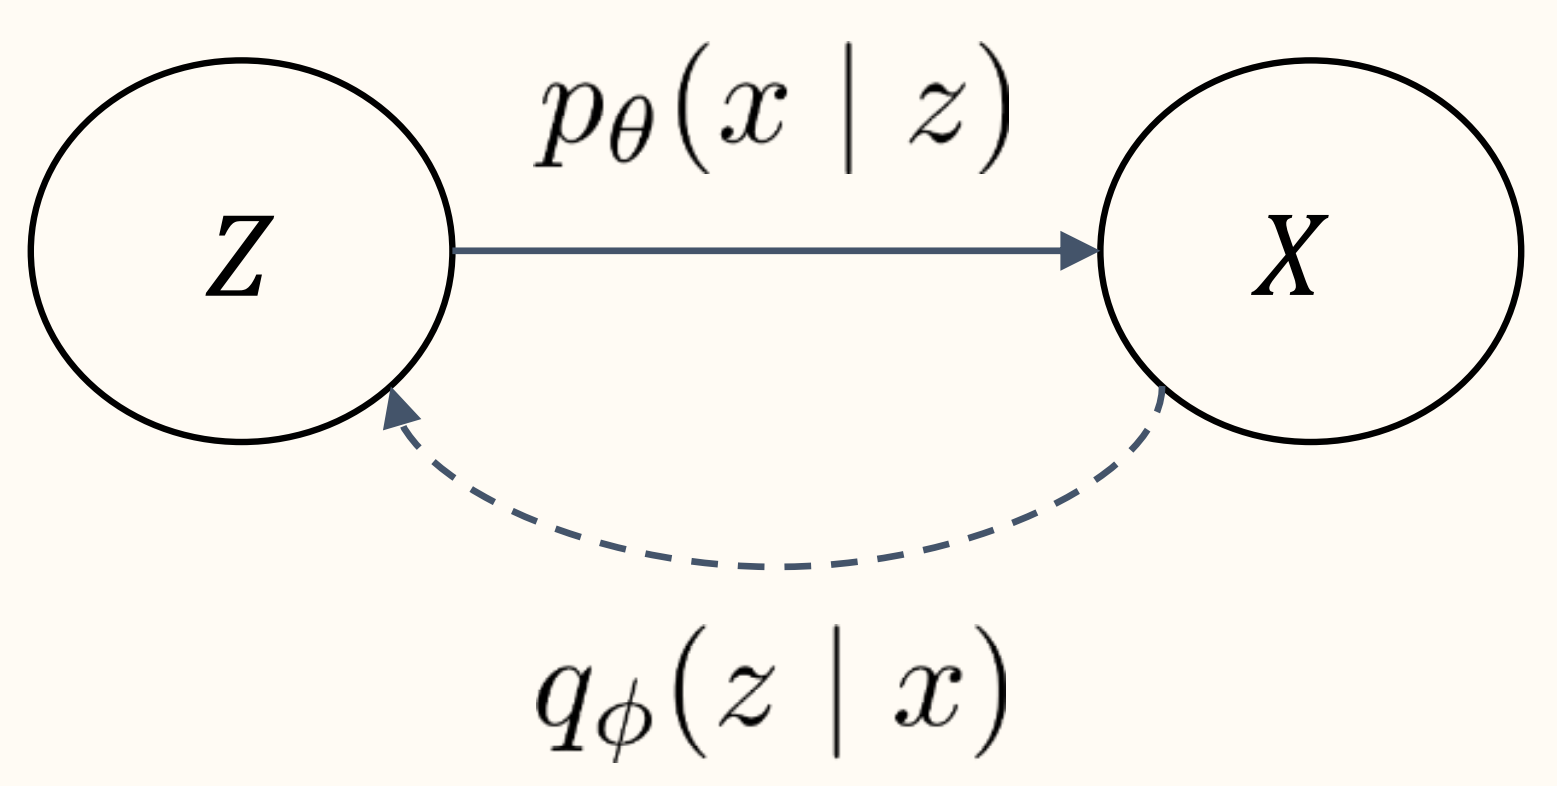
\includegraphics[width=0.5\textwidth]{.././assets/11.4.png}
    \end{figure}

    \begin{itemize}
        \item \textbf{Likelihood} : $\textcolor{red}{p_{\theta}(x)}$ (exact evaluation intractable)
        \item \textbf{Prior} : $p_{Z}(z)$
        \item \textbf{Conditional distribution (decoder)} : $p_{\theta}(x \mid z)$
        \item \textbf{True posterior} : $\textcolor{red}{p_{\theta}(z \mid x)}$ (exact evaluation intractable)
        \item \textbf{Approximate posterior (encoder)} : $q_{\phi}(z \mid x)$
    \end{itemize}

    \par\noindent\textcolor{gray}{\hdashrule{\textwidth}{0.4pt}{1pt 2pt}}

    Conditional distribution $p_{\theta}(x \mid z)$ and prior $p_{Z}(z)$ determines the posterior $p_{\theta}(z \mid x)$.

    There is no easy way to evaluate $p_{\theta}(x)$, but we can sample $X \sim p_{\theta}(x)$ easily: $Z \sim p_{Z}(z)$ then $X \sim p_{\theta}(x \mid Z)$.

    NN in VAE do not directly generate random output. NN outputs parameters for random sampling.
\end{definition}

\section{VAE Standard Instance}

\begin{definition}[11.17][VAE Standard Instance]
    A \textbf{standard VAE setup}:

    $$
    \begin{aligned}
    & p_{Z}=\mathcal{N}(0, I) \\
    & q_{\phi}(z \mid x)=\mathcal{N}\left(\mu_{\phi}(x), \Sigma_{\phi}(x)\right) \text { with diagonal } \Sigma_{\phi} \\
    & p_{\theta}(x \mid z)=\mathcal{N}\left(f_{\theta}(z), \sigma^{2} I\right)
    \end{aligned}
    $$

    $\mu_{\phi}(x), \Sigma_{\phi}^{2}(x)$, and $f_{\theta}(z)$ are deterministic NN.

    \par\noindent\textcolor{gray}{\hdashrule{\textwidth}{0.4pt}{1pt 2pt}}

    Using the following equation,

    $$
    \begin{aligned}
    & D_{\mathrm{KL}}\left(\mathcal{N}\left(\mu_{\phi}(X), \Sigma_{\phi}(X)\right) \| \mathcal{N}(0, I)\right) \\
    = & \frac{1}{2}\left(\operatorname{tr}\left(\Sigma_{\phi}(X)\right)+\left\|\mu_{\phi}(X)\right\|^{2}-d-\log \operatorname{det}\left(\Sigma_{\phi}(X)\right)\right) \\
    \end{aligned}
    $$

    the training objective

    $$
    \underset{\theta \in \Theta, \phi \in \Phi}{\operatorname{maximize}} \sum_{i=1}^{N} \mathbb{E}_{Z \sim q_{\phi}\left(z \mid X_{i}\right)}\left[\log p_{\theta}\left(X_{i} \mid Z\right)\right]-D_{\mathrm{KL}}\left(q_{\phi}\left(\cdot \mid X_{i}\right) \| p_{Z}(\cdot)\right)
    $$

    becomes

    $$
    \underset{\theta \in \Theta, \phi \in \Phi}{\operatorname{minimize}} \sum_{i=1}^{N} \frac{1}{\sigma^{2}} \mathbb{E}_{Z \sim \mathcal{N}\left(\mu_{\phi}\left(X_{i}\right), \Sigma_{\phi}\left(X_{i}\right)\right)}\left\|X_{i}-f_{\theta}(Z)\right\|^{2}+\operatorname{tr}\left(\Sigma_{\phi}\left(X_{i}\right)\right)+\left\|\mu_{\phi}\left(X_{i}\right)\right\|^{2}-\log \operatorname{det}\left(\Sigma_{\phi}\left(X_{i}\right)\right)
    $$
\end{definition}

\begin{concept}[11.18][VAE Standard Instance with Reparameterization Trick]
    The standard instance of VAE

    $$
    \underset{\theta \in \Theta, \phi \in \Phi}{\operatorname{minimize}} \sum_{i=1}^{N} \frac{1}{\sigma^{2}} \mathbb{E}_{Z \sim \mathcal{N}\left(\mu_{\phi}\left(X_{i}\right), \Sigma_{\phi}\left(X_{i}\right)\right)}\left\|X_{i}-f_{\theta}(Z)\right\|^{2}+\operatorname{tr}\left(\Sigma_{\phi}\left(X_{i}\right)\right)+\left\|\mu_{\phi}\left(X_{i}\right)\right\|^{2}-\log \operatorname{det}\left(\Sigma_{\phi}\left(X_{i}\right)\right)
    $$

    can be equivalently written with the reparameterization trick

    $$
    \underset{\theta \in \Theta, \phi \in \Phi}{\operatorname{minimize}} \sum_{i=1}^{N} \frac{1}{\sigma^{2}} \mathbb{E}_{\varepsilon \sim \mathcal{N}(0, I)}\left\|X_{i}-f_{\theta}\left(\mu_{\phi}\left(X_{i}\right)+\Sigma_{\phi}^{1 / 2}\left(X_{i}\right) \varepsilon\right)\right\|^{2}+\operatorname{tr}\left(\Sigma_{\phi}\left(X_{i}\right)\right)+\left\|\mu_{\phi}\left(X_{i}\right)\right\|^{2}-\log \operatorname{det}\left(\Sigma_{\phi}\left(X_{i}\right)\right)
    $$

    where $\Sigma_{\phi}^{1 / 2}$ is diagonal with $\sqrt{\cdot}$ of the diagonal elements of $\Sigma_{\phi}$.
    (Remember, $\Sigma_{\phi}$ is diagonal.)

    To clarify $Z \stackrel{\mathcal{D}}{=} \mu_{\phi}\left(X_{i}\right)+\Sigma_{\phi}^{1 / 2}\left(X_{i}\right) \varepsilon$, where $\stackrel{\mathcal{D}}{=}$ denotes equality in distribution.

    We now have an objective amenable to stochastic optimization.
\end{concept}

\begin{concept}[11.19][VAE Standard Instance Architecture]
    \begin{itemize}
        \item Training (Without reparameterization trick)
    \end{itemize}

    \begin{figure}[H]
        \centering
        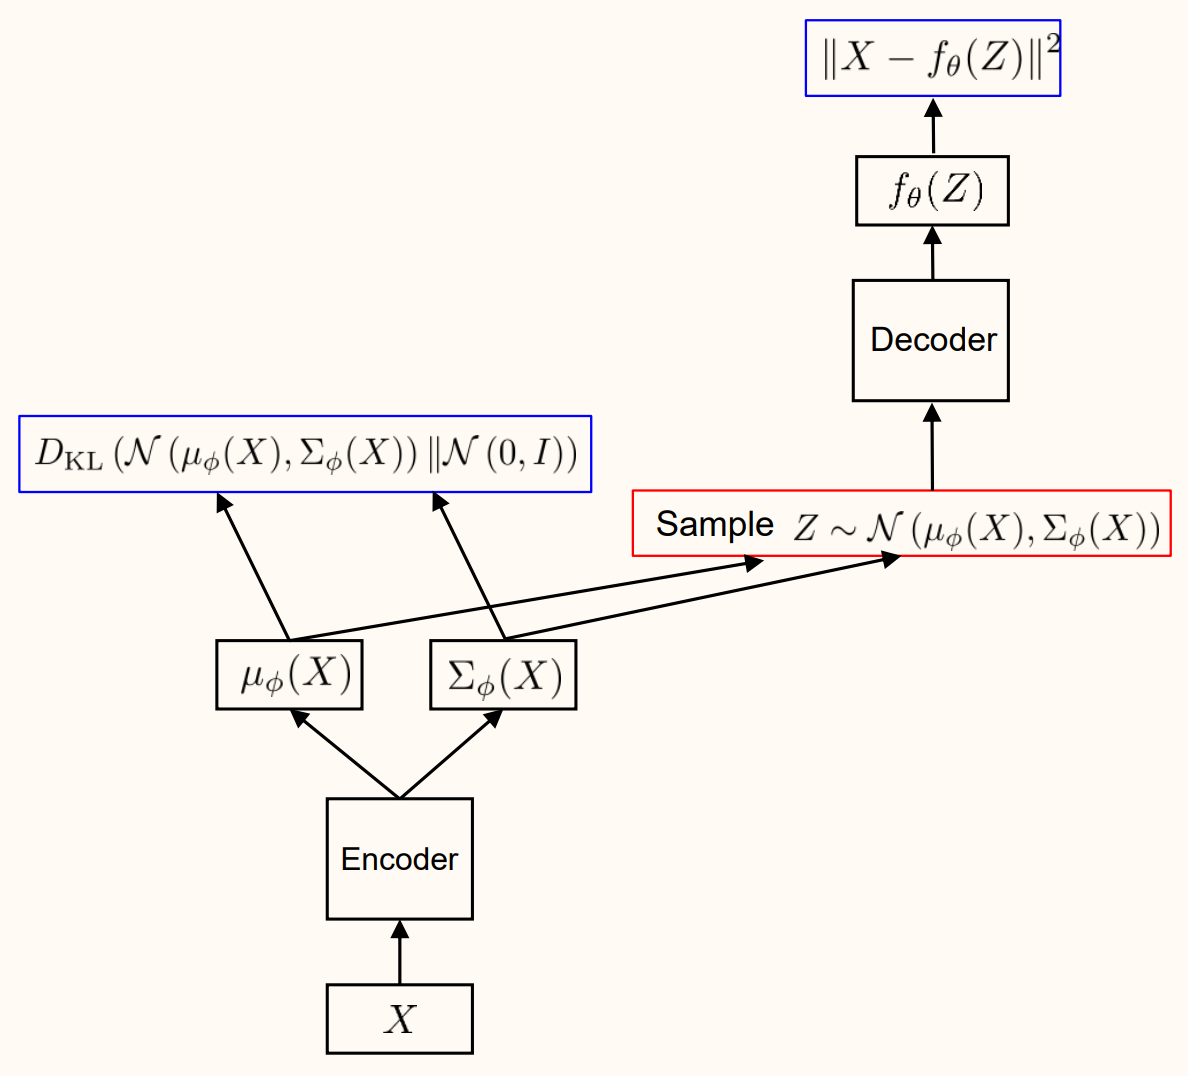
\includegraphics[width=0.7\textwidth]{.././assets/11.5.png}
    \end{figure}

    \begin{itemize}
        \item Training (With reparameterization trick)
    \end{itemize}

    \begin{figure}[H]
        \centering
        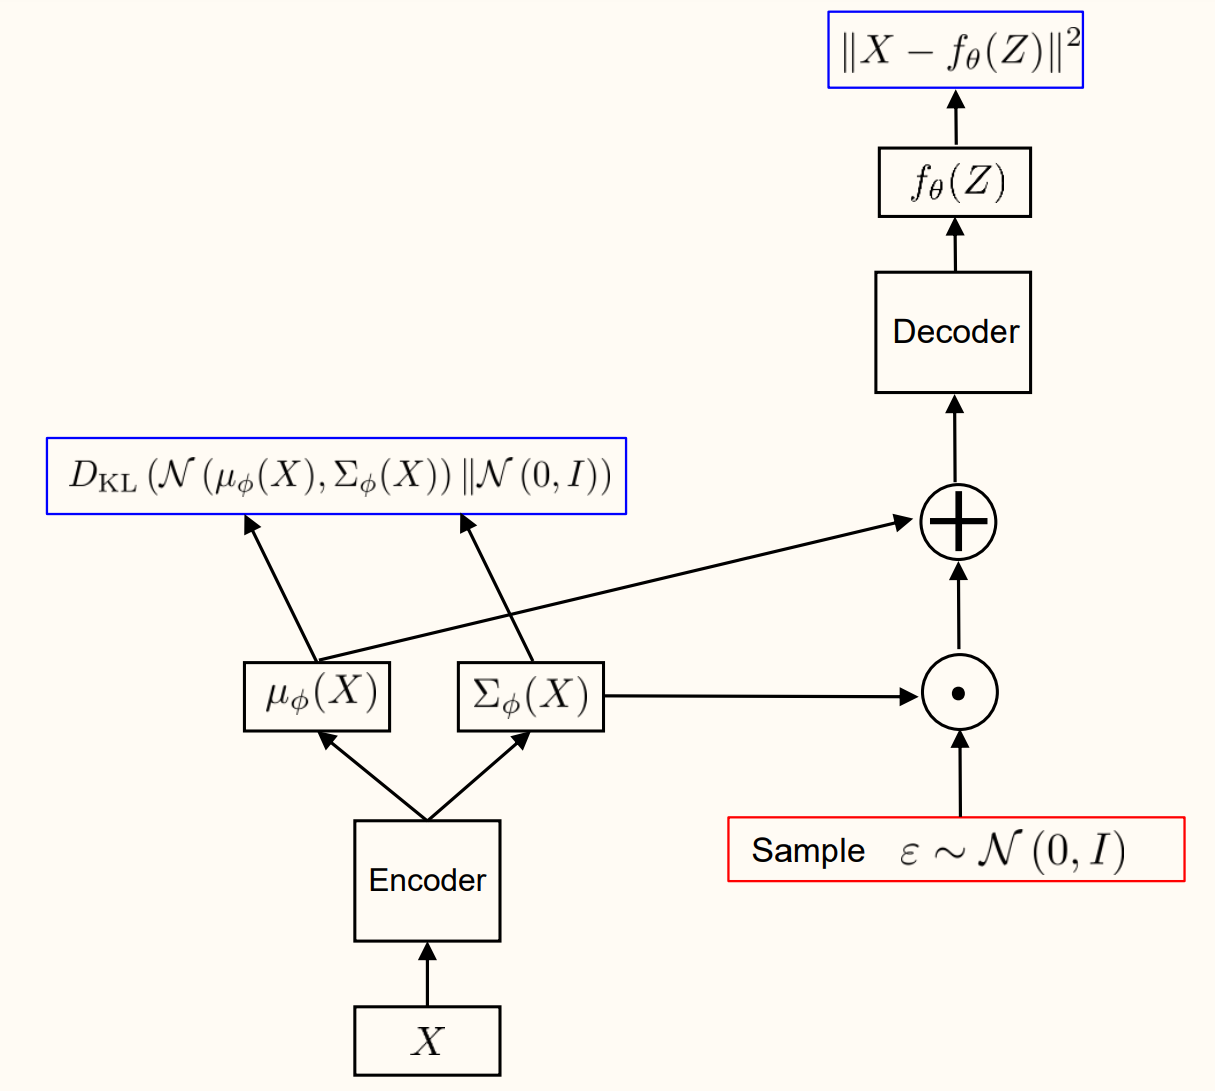
\includegraphics[width=0.7\textwidth]{.././assets/11.6.png}
    \end{figure}

    \par\noindent\textcolor{gray}{\hdashrule{\textwidth}{0.4pt}{1pt 2pt}}

    \begin{itemize}
        \item
        Sampling

        During sampling, only the decoder network is used.
    \end{itemize}

    \begin{figure}[H]
        \centering
        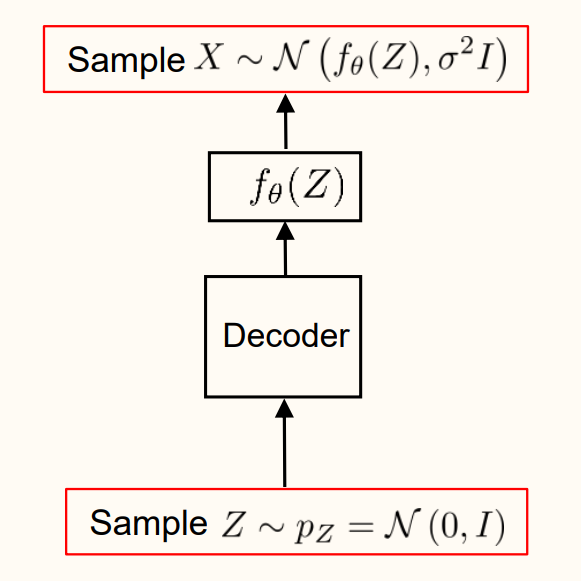
\includegraphics[width=0.4\textwidth]{.././assets/11.7.png}
    \end{figure}
\end{concept}

\begin{concept}[11.20][Why variational]
    VAE loss (VLB) contains a reconstruction loss resembling that of an autoencoder.

    $$
    \begin{aligned}
    \operatorname{VLB}_{\theta, \phi}\left(X_{i}\right) & =\mathbb{E}_{Z \sim q_{\phi}\left(z \mid X_{i}\right)}\left[\log p_{\theta}\left(X_{i} \mid Z\right)\right]-D_{\mathrm{KL}}\left(q_{\phi}\left(\cdot \mid X_{i}\right) \| p_{Z}(\cdot)\right) \\
    & =-\frac{1}{2 \sigma^{2}} \mathbb{E}_{Z \sim q_{\phi}\left(z \mid X_{i}\right)}\left[\left\|X_{i}-f_{\theta}(Z)\right\|^{2}\right]-D_{\mathrm{KL}}\left(q_{\phi}\left(\cdot \mid X_{i}\right) \| p_{Z}(\cdot)\right) \\
    & =-\underbrace{\frac{1}{2 \sigma^{2}} \mathbb{E}_{\varepsilon \sim \mathcal{N}(0, I)}\left\|X_{i}-f_{\theta}\left(\mu_{\phi}\left(X_{i}\right)+\Sigma_{\phi}^{1 / 2}\left(X_{i}\right) \varepsilon\right)\right\|^{2}}_{\text {Reconstruction loss }}-\underbrace{D_{\mathrm{KL}}\left(q_{\phi}\left(\cdot \mid X_{i}\right) \| p_{Z}(\cdot)\right)}_{\text {Regularization }}
    \end{aligned}
    $$

    VLB also contains a regularization term on the output of the encoder, which is not present in standard autoencoder losses.

    The choice of $\sigma$ determines the relative weight between the reconstruction loss and the regularization.
\end{concept}

\section{Training VAE}

\begin{concept}[11.21][Training VAE with RT]
    To obtain stochastic gradients of the VAE standard instance 

    $$
    \underset{\theta \in \Theta, \phi \in \Phi}{\operatorname{minimize}} \sum_{i=1}^{N} \frac{1}{\sigma^{2}} \mathbb{E}_{\varepsilon \sim \mathcal{N}(0, I)}\left\|X_{i}-f_{\theta}\left(\mu_{\phi}\left(X_{i}\right)+\Sigma_{\phi}^{1 / 2}\left(X_{i}\right) \varepsilon\right)\right\|^{2}+\operatorname{tr}\left(\Sigma_{\phi}\left(X_{i}\right)\right)+\left\|\mu_{\phi}\left(X_{i}\right)\right\|^{2}-\log \operatorname{det}\left(\Sigma_{\phi}\left(X_{i}\right)\right)
    $$

    select a data $X_{i}$, sample $\varepsilon_{i} \sim \mathcal{N}(0, I)$, evaluate

    $$
    -\operatorname{VLB}_{\theta, \phi}\left(X_{i}, \varepsilon_{i}\right) \stackrel{\text { def }}{=} \frac{1}{\sigma^{2}}\left\|X_{i}-f_{\theta}\left(\mu_{\phi}\left(X_{i}\right)+\Sigma_{\phi}^{1 / 2}\left(X_{i}\right) \varepsilon_{i}\right)\right\|^{2}+\operatorname{tr}\left(\Sigma_{\phi}\left(X_{i}\right)\right)+\left\|\mu_{\phi}\left(X_{i}\right)\right\|^{2}-\log \operatorname{det}\left(\Sigma_{\phi}\left(X_{i}\right)\right)
    $$

    and backprop on $\operatorname{VLB}_{\theta, \phi}\left(X_{i}, \varepsilon_{i}\right)$.

    Usually, batch of $X_{i}$ is selected.\\
    One can sample multiple $Z_{i, 1}, \ldots, Z_{i, K}$ (equivalently $\varepsilon_{i, 1}, \ldots, \varepsilon_{i, K}$ ) for each $X_{i}$.
\end{concept}

\begin{concept}[11.22][Traning VAE with Log-Derivative Trick]
    Computing stochastic gradients without the reparameterization trick.

    $$
    \underset{\theta \in \Theta, \phi \in \Phi}{\operatorname{maximize}} \sum_{i=1}^{N} \underbrace{\mathbb{E}_{Z \sim q_{\phi}\left(z \mid X_{i}\right)}\left[\log \left(\frac{p_{\theta}\left(X_{i} \mid Z\right) p_{Z}(Z)}{q_{\phi}\left(Z \mid X_{i}\right)}\right)\right]}_{\stackrel{\text { def }}{=} \operatorname{VLB}_{\theta, \phi}\left(X_{i}\right)}
    $$

    To obtain unbiased estimates of $\nabla_{\theta}$, compute

    $$
    \frac{1}{K} \sum_{k=1}^{K} \log p_{\theta}\left(X_{i} \mid Z_{i, k}\right), \quad Z_{i, 1}, \ldots, Z_{i, K} \sim q_{\phi}\left(z \mid X_{i}\right)
    $$

    and backprop with respect to $\theta$.

    We differentiate the VLB objectives

    $$
    \begin{aligned}
    \nabla_{\phi} \mathbb{E}_{Z \sim q_{\phi}\left(z \mid X_{i}\right)}\left[\log \left(\frac{p_{\theta}\left(X_{i} \mid Z\right) p_{Z}(Z)}{q_{\phi}\left(Z \mid X_{i}\right)}\right)\right] & =\nabla_{\phi} \int \log \left(\frac{p_{\theta}\left(X_{i} \mid z\right) p_{Z}(z)}{q_{\phi}\left(z \mid X_{i}\right)}\right) q_{\phi}\left(z \mid X_{i}\right) d z \\
    & =\mathbb{E}_{Z \sim q_{\phi}\left(z \mid X_{i}\right)}\left[\left(\nabla_{\phi} \log q_{\phi}\left(Z \mid X_{i}\right)\right) \log \left(\frac{p_{\theta}\left(X_{i} \mid Z\right) p_{Z}(Z)}{q_{\phi}\left(Z \mid X_{i}\right)}\right)\right]
    \end{aligned}
    $$

    To obtain unbiased estimates of $\nabla_{\phi}$, compute

    $$
    \frac{1}{K} \sum_{k=1}^{K}\left(\nabla_{\phi} \log q_{\phi}\left(Z_{i, k} \mid X_{i}\right)\right) \log \left(\frac{p_{\theta}\left(X_{i} \mid Z_{i, k}\right) p_{Z}\left(Z_{i, k}\right)}{q_{\phi}\left(Z_{i, k} \mid X_{i}\right)}\right), \quad Z_{i, 1}, \ldots, Z_{i, K} \sim q_{\phi}\left(z \mid X_{i}\right)
    $$
\end{concept}

\section{Researches}

\begin{concept}[11.23][VQ-VAE]
    \begin{figure}[H]
        \centering
        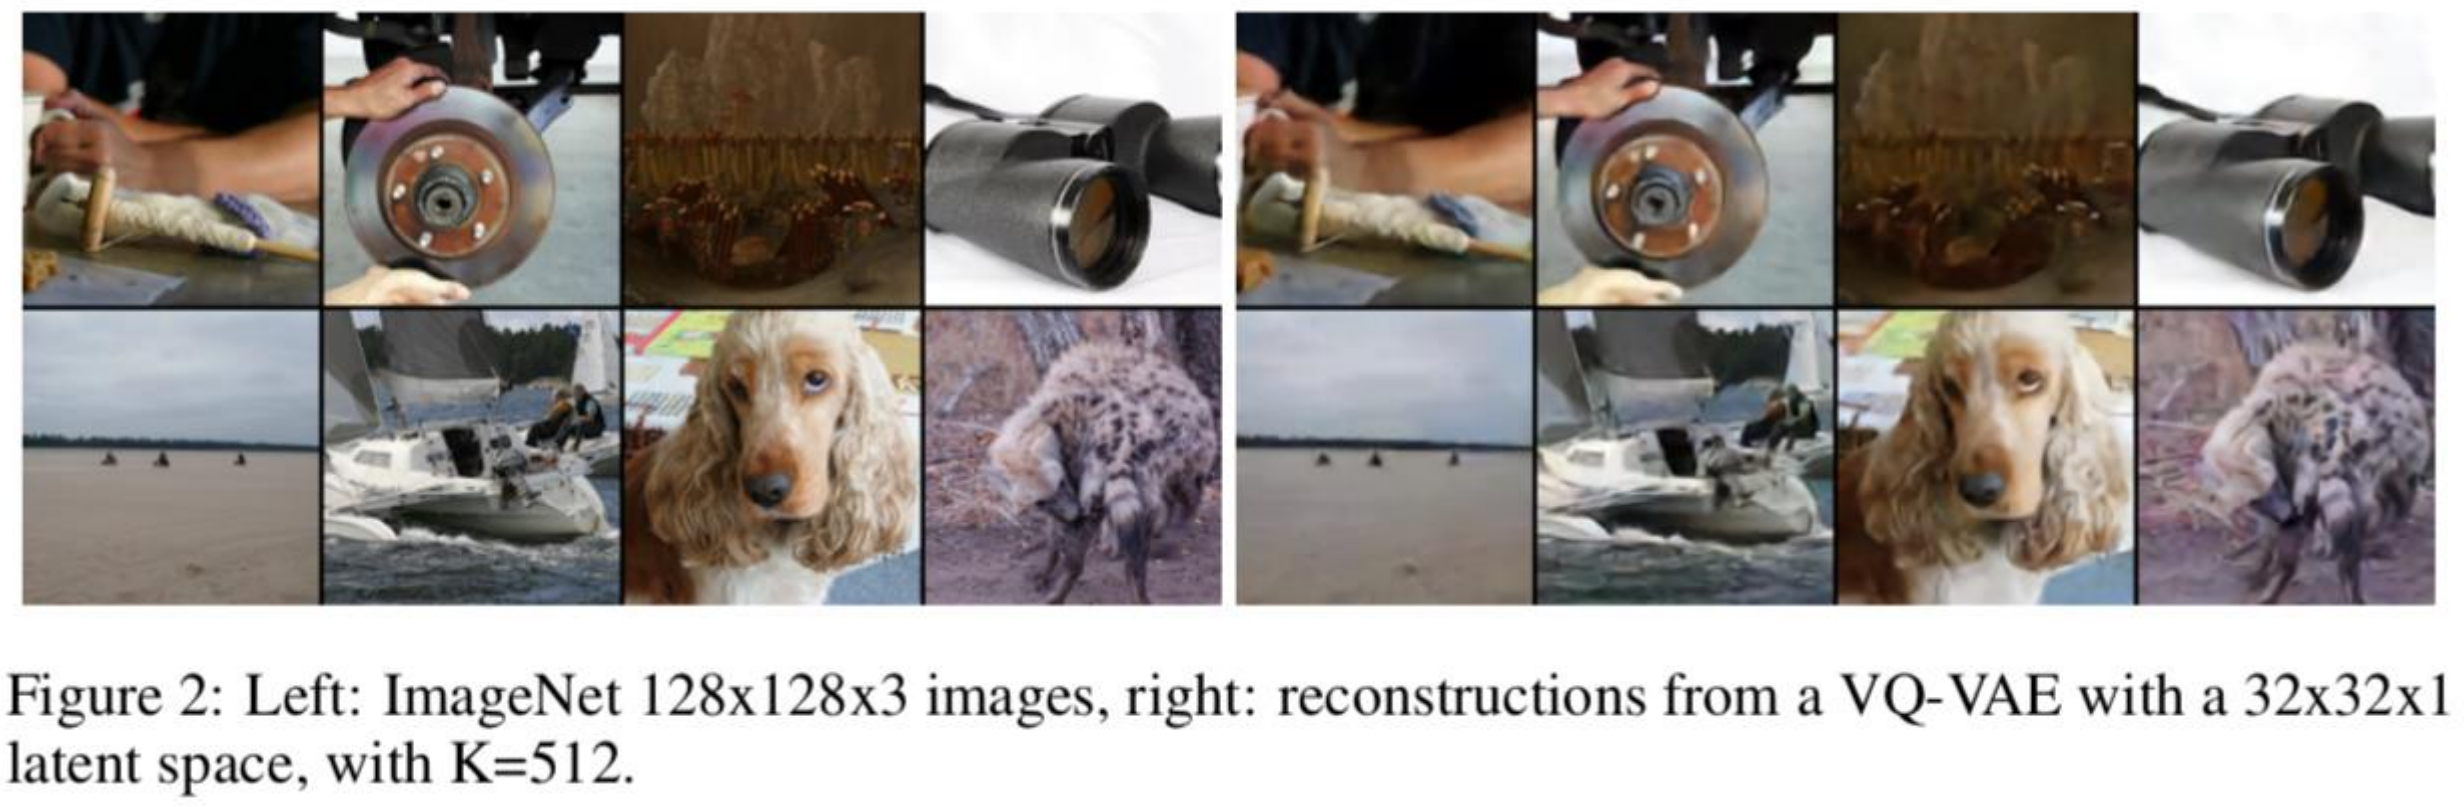
\includegraphics[width=1.0\textwidth]{.././assets/11.8.png}
    \end{figure}

    \begin{figure}[H]
        \centering
        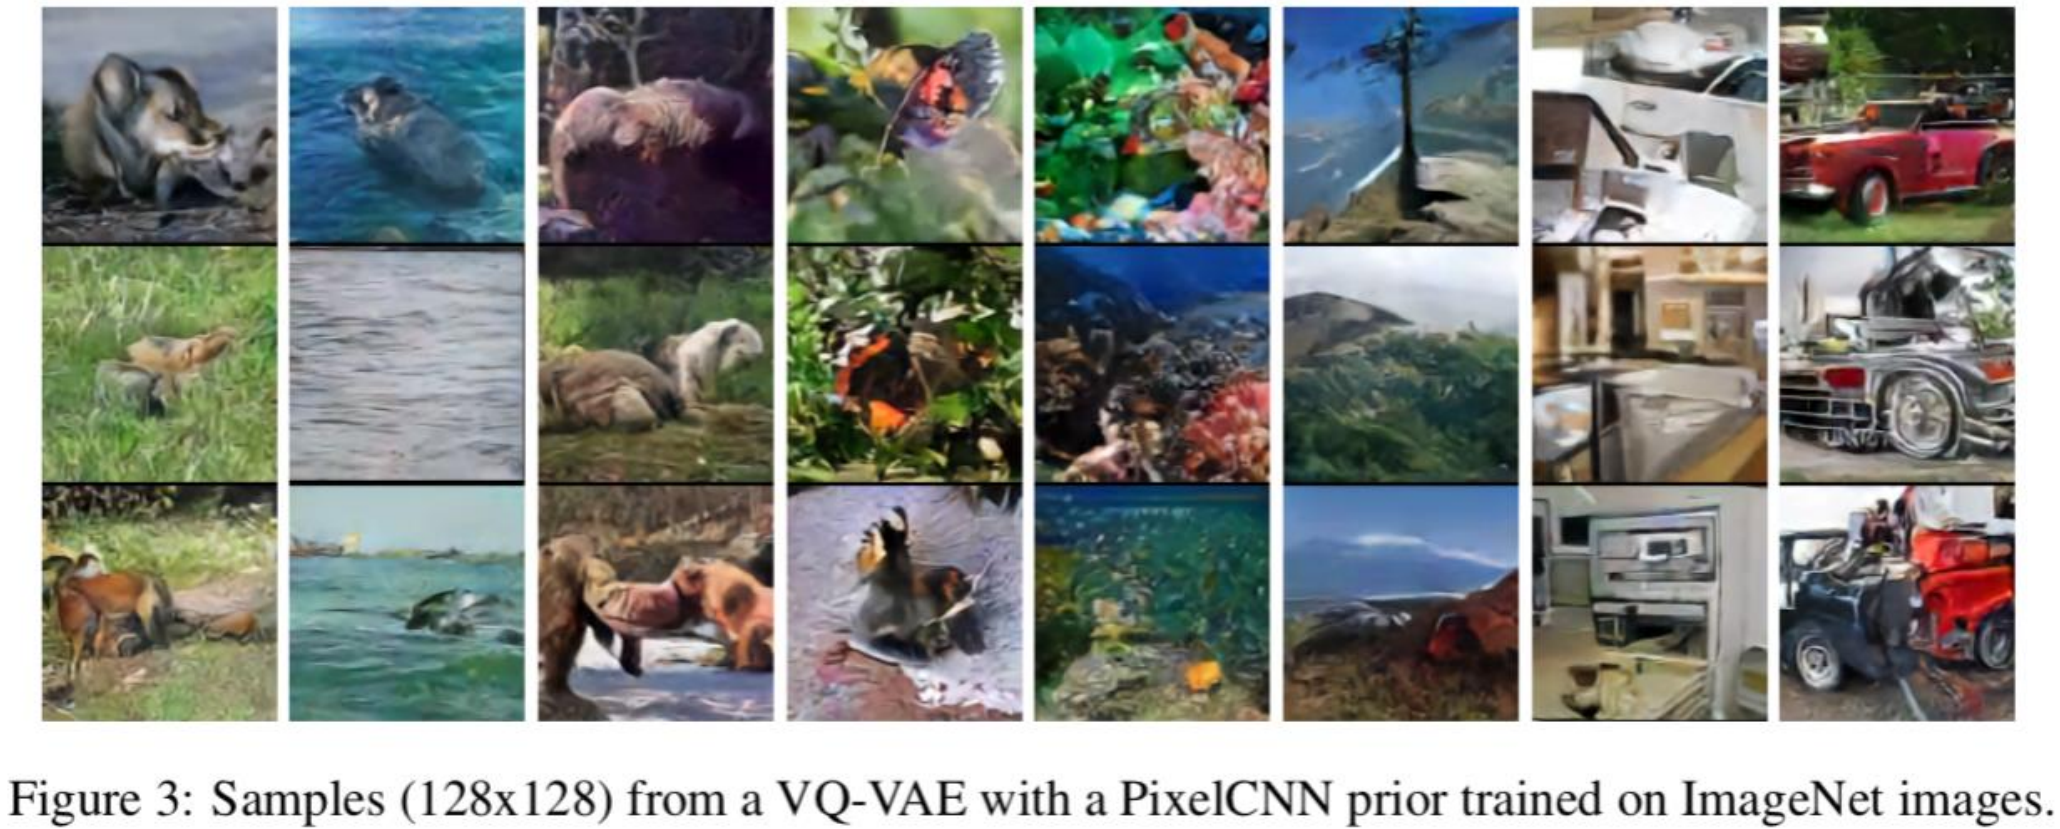
\includegraphics[width=1.0\textwidth]{.././assets/11.9.png}
    \end{figure}

    (A. van den Oord, O. Vinyals, and K. Kavukcuoglu, Neural discrete representation learning, NeurIPS, 2017.)
\end{concept}

\begin{concept}[11.24][VQ-VAE-2]
    \begin{figure}[H]
        \centering
        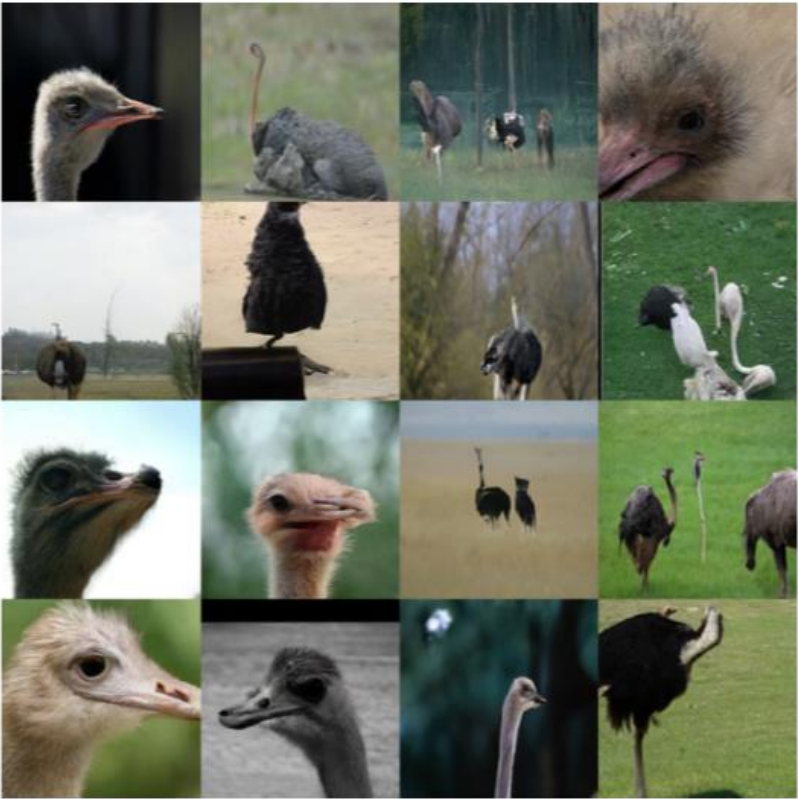
\includegraphics[width=0.5\textwidth]{.././assets/11.10.png}
    \end{figure}

    \begin{figure}[H]
        \centering
        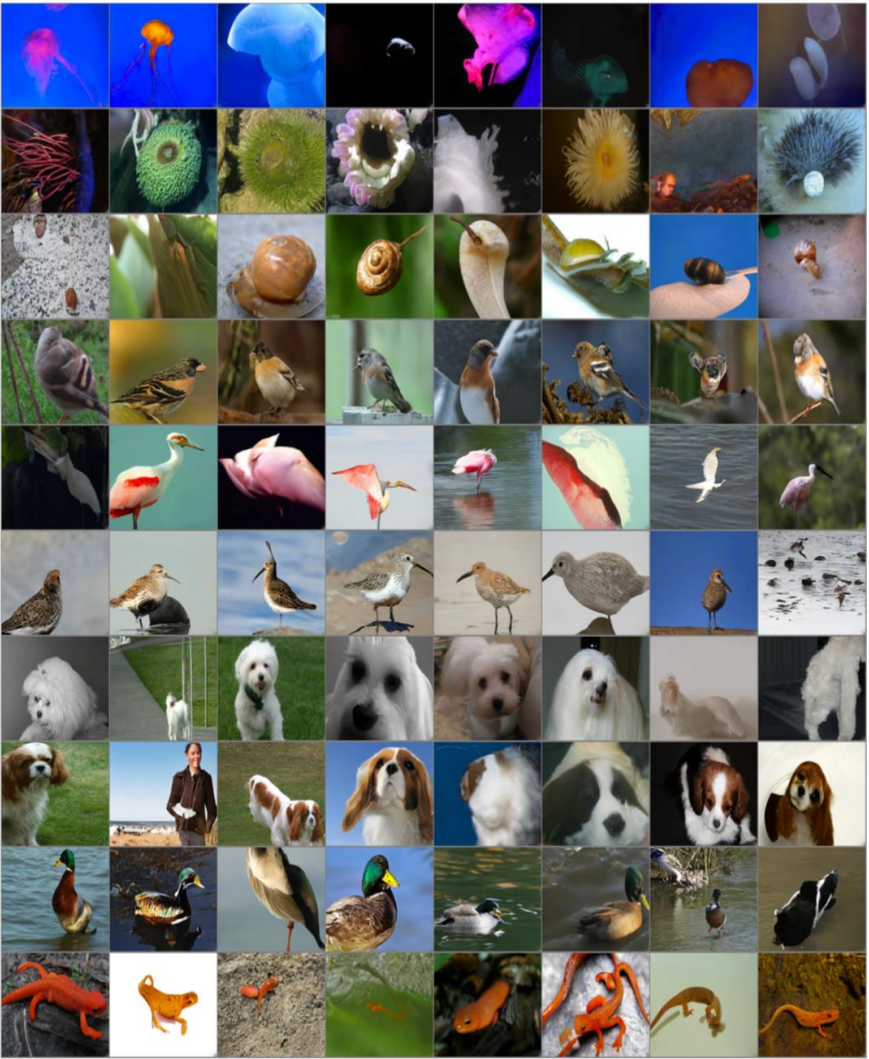
\includegraphics[width=0.7\textwidth]{.././assets/11.11.png}
    \end{figure}

    \begin{figure}[H]
        \centering
        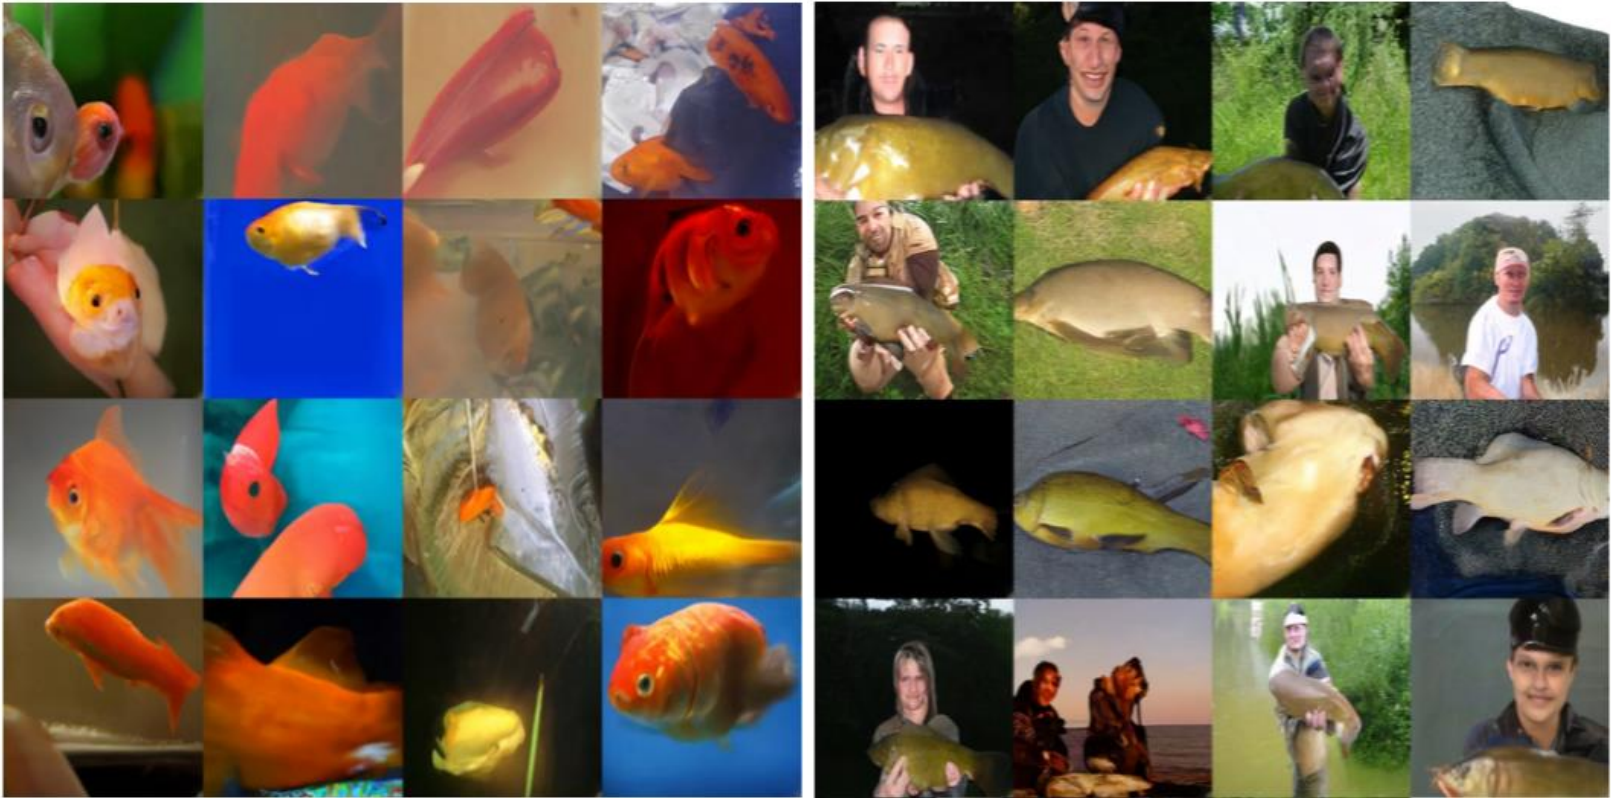
\includegraphics[width=1.0\textwidth]{.././assets/11.12.png}
    \end{figure}

    (A. Razavi, A. van den Oord, and O. Vinyals, Generating diverse high-fidelity images with VQ-VAE-2, NeurIPS, 2019.)
\end{concept}

\begin{concept}[11.25][$\beta$-VAE]
    Uses the loss

    $$
    \ell_{\theta, \phi}\left(X_{i}\right)=\mathbb{E}_{Z \sim q_{\phi}\left(z \mid X_{i}\right)}\left[\log p_{\theta}\left(X_{i} \mid Z\right)\right]-\beta D_{\mathrm{KL}}\left(q_{\phi}\left(\cdot \mid X_{i}\right) \| p_{Z}(\cdot)\right)
    $$

    when $\beta=1, \ell_{\theta, \phi}\left(X_{i}\right)=\operatorname{VLB}_{\theta, \phi}\left(X_{i}\right)$, i.e., $\beta$-VAE coincides with VAE when $\beta=1$.

    With $\beta>1$, authors observed better feature disentanglement.

    (I. Higgins, L. Matthey, A. Pal, C. Burgess, X. Glorot, M. Botvinick, S. Mohamed, and A. Lerchner, β-VAE: Learning basic visual concepts with a constrained variational framework, ICLR, 2017.)
\end{concept}
